\section{Adaptive control strategy}

The intelligent control strategy proposed in this paper is shown in \figref{fig:stepMap}.
\begin{figure}[H]
	\centering
	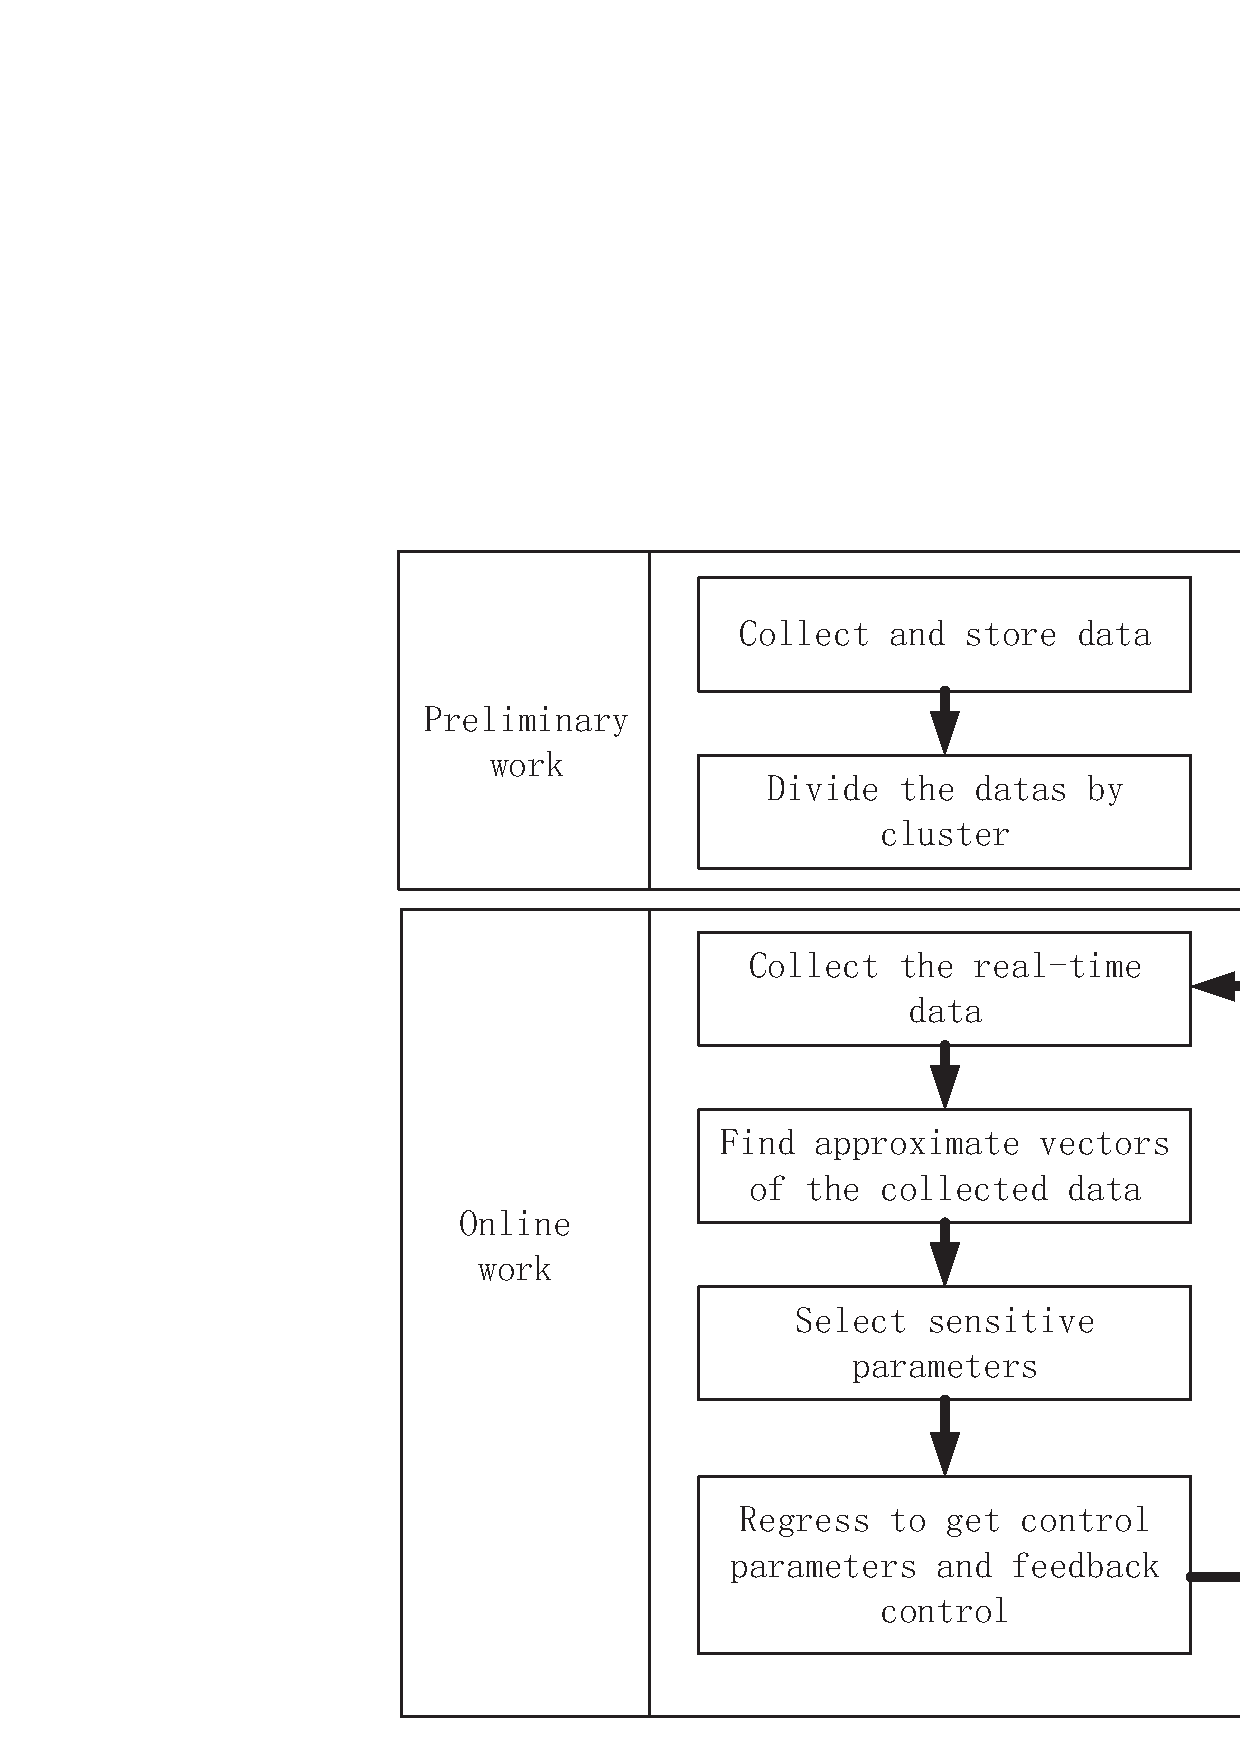
\includegraphics[width=.8\linewidth]{fig/mainwork/stepMap}
	\caption{The overall experimental flow chart}
	\figlabel{fig:stepMap}
\end{figure}

 In the preprocessing work, we let the robot move in different environments for a large number of times and we collect and store the data listed in the form like \figref{fig:data}.
\begin{figure}[H]
	\centering
	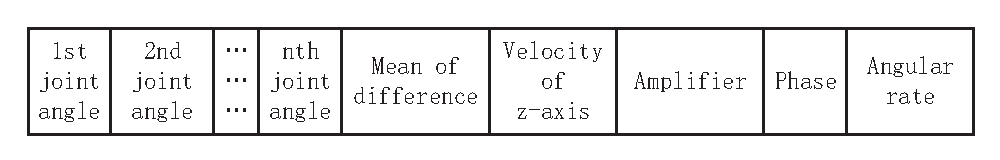
\includegraphics[width=\linewidth]{fig/mainwork/data}
	\caption{The structure of the data storage}
	\figlabel{fig:data}
\end{figure}

In this way, we define "Mean of difference" as $\frac{\sum_{i=1}^{n}(t^{(i)}-ma^{(i)})}{n} $ where n is the number of joints. $T=\begin{bmatrix}
t^{(1)} & t^{(2)} & \cdots & t^{(n)}
\end{bmatrix}$ is the desired joint angles and $MA=\begin{bmatrix}
ma^{(1)} & ma^{(2)} & \cdots & ma^{(n)}
\end{bmatrix}$ is the measured joint angles. The control vector is shown as
$V_C=\begin{bmatrix}
A\\ 
\omega\\
\varepsilon
\end{bmatrix}$
where $A$ is the amplitude, $\omega$ is the phase, and the $\varepsilon$ is the angular rate. All of them come from Eq.\ref{basicRoll}.

After collecting movement data of a snake-like robot, we cluster the training data in order to simplify the data processing.

In robot's running time, we get the real-time data periodically and then we do the following steps. Firstly, we categorize the real-time data based on the clustering result in preprocessing. And then we select the most sensitive gait parameter according to the entropy variance. At last, we use the idea of regression to modify the sensitive gait parameter and keep the other gait parameters unchanged.

\subsection{Implementation of Clustering by $Kmeans++$}
In this research, collected data in preprocessing is a large-scale data set. As $kmeans++$ algorithm has high efficiency and scalability for a large-scale data set, we adopt $kmeans++$ for clustering. We classify training set into $N_{k}$ blocks. The clustering process is divided into the following steps:

\begin{itemize}
	\item Step 1: Randomly select a point in the training set as the first cluster center.
	\item Step 2: For the $k_{th}$ center, select the point which has the largest  distance to the $(k-1)$ centers in the current training set
	%prework step2
	\begin{eqnarray}\label{clu_step2}
	\left\{
	\begin{array}{lr}
	F_{c}\left ( P^{\left (  i\right )} \right ) = \sum_{j=1}^{k-1}\left \| X^{\left ( j-1 \right )}-P^{\left (  i\right )} \right \|_{2}\\
	k = $arg$\max \limits_{i}{(F_{C}(P^{(i)}))}
	\end{array}
	\right.
	\end{eqnarray}
	\begin{figure}[H]
		\centering
		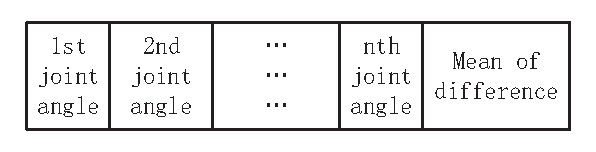
\includegraphics[height=0.5in]{fig/mainwork/data2}
		\caption{Data vector used in clustering and regression}
		\figlabel{fig:data2}
	\end{figure}
	$P^{(i)}$ is a data(\figref{fig:data2}) in the training set. $X^{(j)}$ is the $j_{th}$ cluster center. $S^{(P)}$ is the  training set. For the initial cluter center $X^{(k)}$, we have $X^{(k)}\in S^{(P)}$ and $X^{(k)}$ is the vector $P^{(i)}$ which corresponds to the result of Eq.\ref{clu_step2}. 
	\item Step 3: Repeat Step 1 and Step 2 until $N_{k}$ cluster centers have been confirmed.
	\item Step 4: After confirming $N_{k}$ cluster center, we categorize every vector in training set based on Eq.\ref{clu_step4}.
	%prework step4
	\begin{eqnarray}\label{clu_step4}
	C^{(i)} = arg\min \limits_{k}{(||P^{(i)}-X^{(k)}||_{2})}
	\end{eqnarray}
	In this equation, $C^{(i)}$ is the flag of category which the vector $P^{(i)}$ belongs to.
	\item Step 5: Refresh the cluster centers according to clustering result by the Eq.\ref{clu_step5}
	%prework step5
	\begin{eqnarray}\label{clu_step5}
	X^{(k)}=\frac{\sum_{i}\{C^{(i)}=k)\}P^{(i)}}{\sum_{i}\{C^{(i)}=k\}}
	\end{eqnarray}
	\item Step 6: iterate Step 4 and 5 until the cluster centers change within a predefined tolerance range.
\end{itemize}

After finishing the clustering, the result is stored in two parts:

\begin{itemize}
	\item The corresponding relationship between each vector in training set and the center of the cluster it belongs to.
	\item The data vectors of each cluster center.
\end{itemize}

With $Kmeans++$, the collected data can be divided into several clusters.

\subsection{Parameter selection by entropy variance}

%classification
\subsubsection{Real-time data categorization}

Every time we get the real-time data, we relegate it to the certain cluster by Eq.\ref{cluster}.
\begin{eqnarray}\label{cluster}
C=arg\min \limits_{k}{(||X^{(k)}-P_{t}||_{2})} \, ,&X^{(C)}\in S^{(X)}
\end{eqnarray}

$S^{(X)}$ is the cluster center set. $X^{(C)}$ is the closet vector to the real-time vector $P_t$. And $X^{(k)}$ is the $i_{th}$ cluster center of the cluster center set $S^{(X)}$ . With $Euclidian \; Distance \; Formula$, we make a prediction on the similarity between two vectors.

\subsubsection{The selection of the preponderant data}

After categorization of real-time data, we select those preponderant vectors whose Z-axis velocity are bigger than current (Eq.\ref{preponderant}).
%find out preponderant
\begin{eqnarray}\label{preponderant}
S^{(V)}=\{P^{(i)}|V_{z}^{(i)}\geq V_{z}^{P_{t}} \; , \; P^{(i)}\in S^{(C)}\}
\end{eqnarray}

$S^{(C)}$ is all the vectors which belong to the cluster with the cluster center $X^{(C)}$. $V_{z}^{(i)}$ is the vertical velocity component of the vector $P^{(i)}$ and $V_{z}^{(P_{t})}$ is the vertical velocity component of the real-time data vector. $S^{(V)}$ is the set of all the preponderant vectors for regression.

\subsubsection{The selection of the sensitive parameter}

We adopt entropy variance as the reference to select the parameter which should be modified. The steps of selecting the sensitive parameter are as follows.

\begin{itemize}
	\item Step 1: We take the preprocessing operation to discrete the preponderant data (Eq.\ref{quantification}).
	%quantification
	\begin{eqnarray}\label{quantification}
	V_{new}^{(i)}=\left\{
	\begin{array}{lr}
	\left \lfloor \frac{V_{z}^{(i)}}{L_{D}} \right \rfloor&V_{z}^{(i)}> 0\\
	\\
	\left \lceil \frac{V_{z}^{(i)}-L_{D}}{L_{D}} \right \rceil&V_{z}^{(i)}\leq 0
	\end{array}
	\right.
	\end{eqnarray}
	
	In Eq.\ref{quantification}, $L_{D}$ is the adjustable step length for discretization. We eventually get the velocity discrete sequence:
	\begin{eqnarray}\label{newMember}
	V_{new}^{(Z)}=\begin{bmatrix}
	V_{new}^{(1)} & V_{new}^{(2)} & V_{new}^{(3)} & V_{new}^{(4)} & \cdots & \cdots
	\end{bmatrix}
	\end{eqnarray}
	
	\item Step 2: There are a variety of possible values for each gait parameter. Thus, in order to record all the possible values, we make a set $S_{ij}^{(P)}$ which is the data set of $j_{th}$ possible value of the gait parameter $i$. And value of $i$ is from 0 to 2 corresponding to amplitude, phase and angular rate respectively. We calculate the entropy about the vertical velocity of the $j_{th}$ possible value of the gait parameter $i$ by Eq.\ref{entropy} as well as the entropy variance of the gait parameter $i$ by Eq.\ref{var_entropy}. In Eq.\ref{entropy}, $p(v_{z})$ is the appearance rate of each member in the velocity discrete sequence as Eq.\ref{newMember}. In Eq.\ref{var_entropy}, $E_{ij}^{(H)}$ is the mean of velocity of  the $j_{th}$ possible value of the gait parameter $i$ and $N_{i}$ is the number of possible values of the gait parameter $i$.
	%entropy
	\begin{eqnarray}\label{entropy}
	H(S_{ij}^{(P)})=-\sum _{v_{z}\in V_{new}^{(Z)}}p(v_{z})log_{2}p(v_{z})
	\end{eqnarray}
	
	%entropy variance
	\begin{eqnarray}\label{var_entropy}
	Var_{i}^{(H)}=\frac{\sum _{N_{i}}(H(S_{ij}^{(P)})-E_{ij}^{(H)})^{2}}{N_{i}}
	\end{eqnarray}
	
	\item Step 3: We normalize the entropy variance (Eq.\ref{normalize}) and randomly select the sensitive gait parameters by roulette method (\figref{fig:Roulette}) to avoid the selection getting stuck in the high probability event.
	%normalize entropy variance
	\begin{eqnarray}\label{normalize}
	R_{i}^{(var)}=\frac{Var_{i}^{(H)}}{\sum Var^{(H)}}
	\end{eqnarray}
	
	\begin{figure}[H]
		\centering
		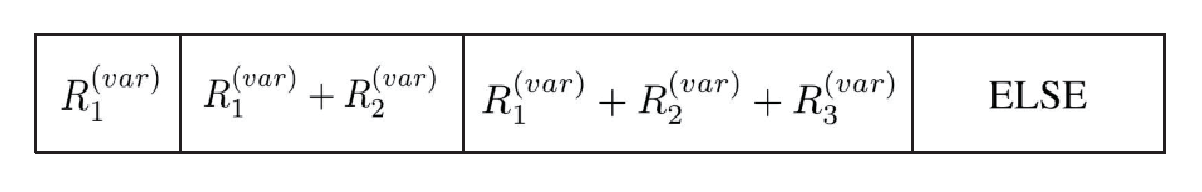
\includegraphics[width=\linewidth]{fig/mainwork/Roulette}
		\caption{Sensitive parameter selection by roulette method}
		\figlabel{fig:Roulette}
	\end{figure}
\end{itemize}

After the calculation of gait parameters' entropy variance. the sensitive parameter will be found. And then the selected parameter is used in the regression control later.


\subsection{Assignment of the sensitive parameter by weighted regression}

In this research, we take weighted regression to get the value of the sensitive gait parameter and use the gradient descent method to solve the weighted least squares problem in fitting regression function.

\begin{itemize}
	\item Step 1: List the fitting prediction function(Eq.\ref{fitfunction})
	%fitting and estimation function
	\begin{eqnarray}\label{fitfunction}
	F_{w}(P_{t})=W^{T}P_{t}\,,&W=\begin{bmatrix}w_{1}\\ w_{2}\\ \vdots \\ w_{m}\end{bmatrix}
	\end{eqnarray}
	
	In Eq.\ref{fitfunction}, $W$ is the coefficient sequence of the fitting equation and $m$ is the number of coefficients where $P_{t}$ is the collected vector in real-time with the model of  \figref{fig:data2}. Then we can get the error function(Eq.\ref{estimate}) which takes the square of error as the estimation with $n$ being the number of data of $S^{(V)}$ and $Q$ being the vector consisting of the sensitive parameter component of the vector $P^{(i)}( P^{(i)} \in P)$.
	%Square sum as an estimation
	\begin{eqnarray}\label{estimate}
		D(W)=\frac{1}{2n}(F_{w}(P)^{T}-Q)^{T}(F_{w}(P)^{T}-Q)
	\end{eqnarray}
	\begin{eqnarray}
		P=\begin{bmatrix}P^{(1)}&P^{(2)}  &\cdots  &P^{(n)} \end{bmatrix}, &P^{(i)}\in S^{(V)}
	\end{eqnarray}
	\begin{eqnarray}
		Q=\begin{bmatrix}Q^{(1)}& Q^{(2)}& \cdots & Q^{(n)}\end{bmatrix}^{T}
	\end{eqnarray}
	
	To get the best-fit coefficient sequence $W$ by the minimum $D(w)$, according to gradient descent method, we turn the Eq.\ref{estimate} into Eq.\ref{Gradde}.
	%Gradient descent
	\begin{eqnarray}\label{Gradde}
	\nabla_{w}D=\frac{1}{n}P(F_{w}(P)^{T}-Q)
	\end{eqnarray}
	
	\item Step 2: Perform the weighted operation on preponderant data vector to ensure the estimate result of fitting is good (Eq.\ref{WeiGradde}).
	%weighted gradient
	\begin{eqnarray}
	\nabla_{w}D=\frac{1}{n}PM(F_{w}(P)^{T}-Q)
	\end{eqnarray}
	\begin{eqnarray}\label{WeiGradde}
	M=\begin{bmatrix}
	\frac{V_{z}^{(1)}}{L_{s}}&0&\cdots&0\\
	0&\frac{V_{z}^{(2)}}{L_{s}}&\ddots&0\\
	\vdots&\ddots&\ddots&0\\
	0&\cdots&0&\frac{V_{z}^{(n)}}{L_{s}}
	\end{bmatrix}
	\end{eqnarray}
	In Eq.\ref{WeiGradde}, $L_s$ is the learning step and $M$ is the learning rate matrix.
	
	\item Step 3: Fit the coefficient vector by Eq.\ref{fit}.
	%fitting the parameters
	\begin{eqnarray}\label{fit}
	W=W-\nabla_{w}D
	\end{eqnarray}
	
	In this way, the coefficient sequence $W$ is updated. And then we assign the predicting result to the sensitive parameter(Eq.\ref{result}).
	%compensation result
	\begin{eqnarray}\label{result}
	Q=F_{w}(P_{t})=W^{T}P_{t}
	\end{eqnarray}
	After this the new predicting result is produced.
	
	\item Step 4: Iterate the steps above until we acquire the best-fit coefficient. The value of $W$ is stable finally.
\end{itemize}

When the iteration is stopped, the best-fit coefficient $W_{best}$ will be obtained. By applying $W_{best}$ to Eq.\ref{result}, we can get the regression value of the sensitive parameter. This value will be used in the robot control. It is worth noting that we only modify the sensitive parameter and others remain the same value.